\subsection{Aufbau}
In Abb.2 ist der erste Aufbau dargestellt, dieser wird für die erste Justierung benötigt und ist ein noch nicht gekoppelter Schwingkreis, bestehend aus einem Sinusgenerator für die Anregung, einer Kapazität und einer Induktivität, sowie einem 48$\Omega$ Widerstand an dem mit dem Oszilloskop die Spannung abgenommen wird. Zusätzlich wird noch eine Verbindung in den X-Eingang des Oszilloskops gelegt, was notwendig ist um mit Hilfe der Lissajous-Figuren Aussagen zu treffen. \\
In Abb.3 wird nun ein zusätzlicher Schwingkreis mit Hilfe von einem Kondensator $C_K$ gekoppelt und dann mit einem Rechtecksignal angeregt. Zu erwähnen ist noch, dass beim tatsächlichen Versuch wieder ein 48$\Omega$ Widerstand verwendet wird. \\
Beim letzten Aufbau (Abb.4) wird nun an den gekoppelte Schwingkreis ein Wobbelgenerator angeschlossen, dieser erzeugt ein Gleichspannungssignal, welches proportional zur Momentanfrequenz ist, ein XY-Schreiber existiert zwar nicht, jedoch lässt sich auch ein Bild am Oszilloskop erzeugen.

\subsection{Messung}
Zu erst wird die Schaltung (Abb.2) nachgebaut um dann die Resonanzfrequenz des abgestimmten Schwingkreises zu ermitteln, dies geschieht unter zu Hilfenahme der Lissajous-Figuren. \\
Danach wird der Schwingkreis mit einem über den Generator erzeugten Rechtecksignal zum Schwingen angeregt. (In Abb.3 illustriert)
Bei der nun folgenden Messung wird für verschiedene $C_K$ das Verhältnis der Schwingungs- und Schwebungsfrequenz ermittelt.
Im nächsten Schritt wird der Rechteck- durch einen Sinusgenerator ersetzt und die Frequenzen $v^+$ und $v^-$ werden in Abhängigkeit von $C_K$ mit Hilfe der Lissajous-Figuren gemessen bei denen die Frequenz 0 oder $\pi$ ist. \\
Zu Letzt wird gemäß Abb.4 eine Schaltung erstellt und am Oszilloskop die entstandenen Bilder abgenommen. 
\begin{figure}[h]
        \centering
        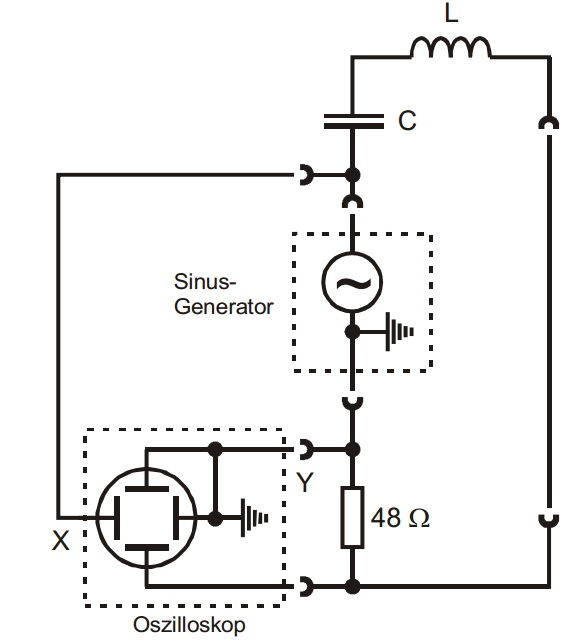
\includegraphics[scale=0.5]{Grafiken/V355Abb2.jpg}
        \caption{Messschaltung zur genauen Bestimmung der Resonanzfrequenz eines Schwingkreises \cite{V355}}
        \label{fig:Abb2}
\end{figure}
\begin{figure}[h]
        \centering
        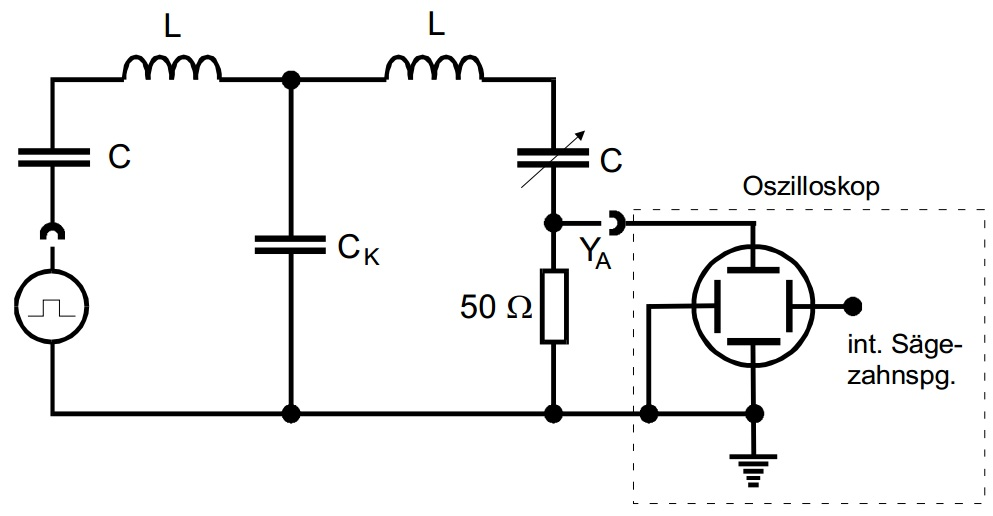
\includegraphics[scale=0.5]{Grafiken/V355Abb3.jpg}
        \caption{Schaltung zur Untersuchung von Schwebungsvorgängen in einem gekoppelten System \cite{V355}}
        \label{fig:Abb3}
\end{figure}
\begin{figure}[h]
        \centering
        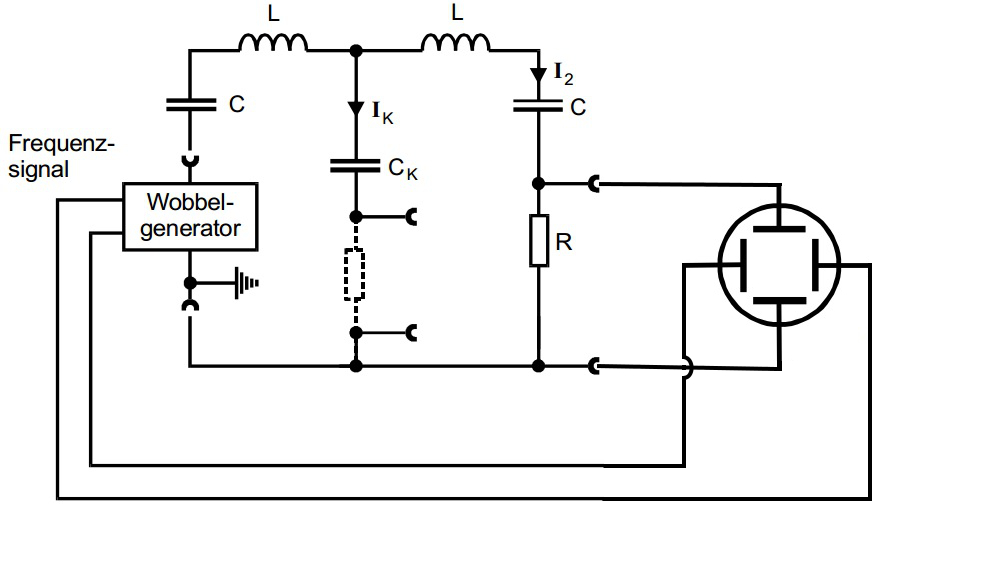
\includegraphics[scale=0.5]{Grafiken/V355Abb4.jpg}
        \caption{Schaltung zur Aufnahme von Stromkurven (bearbeitet)\cite{V355}}
        \label{fig:Abb4}
\end{figure}
